Математическая оптимизация это современное и активно развивающееся направление исследований, определяющее
выбор оптимальных параметров для максимизации результата. Теория оптимизации широко применяется в экономике,
теории игр и физике для разрешения важных практических постановок управления системами и их проектирования. 
Задачи оптимизации классифицируются по наличию ограничений на аргументы функции, виду отклика и постановке задачи. 
Для каждой специфичной постановки, как правило, существует специальная теория, адаптирующая базовый аппарат 
оптимизации под конкретную задачу. Общими же являются методы, использующие производные оптимизируемой функции для поиска 
численной схемы, обеспечивающей эффективный поиск экстремума.

Современная задача оптимизации с учетом ошибки наблюдения записывается как \cite{nesterov2015universal}:
\begin{equation}
    f(x) = \mathrm{E} f(x,\xi) \rightarrow \min_x,
\end{equation}
где пара $(x,\xi)$ является результатом наблюдения с детерминированным параметром $x$ и случайной величиной $\xi$.
В секции для упрощения будут рассмотрены только методы первого порядка.

\text{Определение:} Функция $f$ называется $L$-липшицевой для метрики $\rho$, 
если $\forall x,y \rightarrow \rho(f(x),f(y)) \le L \cdot \rho(x,y)$.
Для оптимизации в качестве метрики, как правило, выбирают эвклидово расстояние $\rho(x,y) =\|x-y \|^2$, задающее 
сходимость по вероятности нормального распределения:   
\begin{equation}
    |f(x) - f(y)| \le L \cdot (x-y)^2
\end{equation}

\textit{Определение:} $\mu$-гладкой называется f(X) функция, для которой выполнено:
\begin{equation}
   \forall x_1,x_2 \in S \rightarrow f(\lambda x_1 + (1-\lambda)x_2) \le \lambda f(x_1) + (1-\lambda) f(x_2) - \frac{\mu}{2} \lambda (1-\lambda) \| x_1 - x_2 \|^2,
\end{equation}
где $S$ --- выпуклое множество и $\mu > 0$. 

\begin{figure}[h]
    \centering
    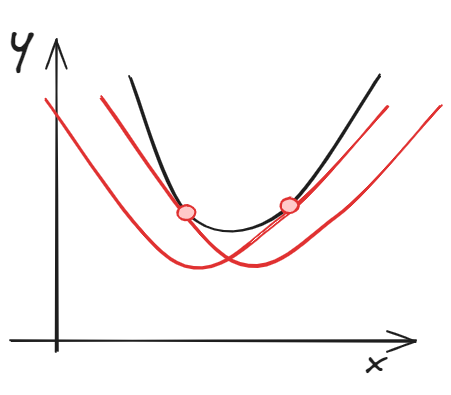
\includegraphics[width=0.5\textwidth]{assets/math/optimization/strong_convex.excalidraw.png}
    \caption{Сильная выпуклость позволяет выполнить квадратичную оценку снизу}
    \label{strong_convex}
\end{figure}

Для выпуклых функций справедливо неравенство Йенсена, широко применяющееся для задания оценки снизу на скорость 
сходимости численной схемы:
\begin{equation}
    f \left( \sum_{i=1}^k \alpha_i x_i \right) \le \sum_{i=1}^k \alpha_i f(x_i),
\end{equation}
причем равенство выполняется только при $x_1 = \dots =x_k$.

Практически важным для выпуклой функции является величина ее матожидания:
\begin{equation}
    f(\mathbb{E} X) \le \mathbb{E} f(X)
\end{equation}

Для современных постановок задач с большими данными существенно исключение стохастического шума. Базовым методом
оптимизации в условиях случайного отлика является усреднение по подвыборке (\textit{англ.} --- batch). 
l
\textit{Определение:} \textbf{Усредненным по подвыборке} мощности $B$ стохастическим градиентом называется 
$\nabla^B f(x,\xi) = \sum_{j=i}^B \nabla f(x,\xi_i)$.

Техника усреднения на шаге приобрела популярность с развитием технологий распределенных вычислений, позволяющих выполнять
расчет параллельно на нескольких вычислителях. Такая методика позволяет ускорить обучение за счет 
проведения большего объема вычислений на каждом шаге расчета.



